\documentclass[12pt,aspectratio=169,ignorenonframetext]{ltxbeamer}

\usepackage[spanish,es-nodecimaldot,es-tabla]{babel}

\title{El universo {\lmr\LaTeX}}
\subtitle{Curso de {\lmr\LaTeX}}
\author{Joar Buitrago\texorpdfstring{\thanks{jebuitragoc@unal.edu.co}}{ <jebuitragoc@unal.edu.co>}}
\date{}

\addbibresource{bibliography.bib}



\begin{document}
\begin{frame}
\maketitle
\end{frame}


\section{Contacto}
\begin{frame}
\begin{columns}
    \begin{column}{0.5\linewidth}
        \centering
        \includegraphics[width=0.75\linewidth]{assets/PillFall_QR.pdf}

        Joar Buitrago
    \end{column}

    \begin{column}{0.5\linewidth}
        \centering
        \includegraphics[width=0.75\linewidth]{assets/repository_QR.pdf}

        github.com/PillFall/Curso-LaTeX
    \end{column}
\end{columns}
\end{frame}


\section{Información del Curso}
\begin{frame}
\frametitle{Información del Curso}

\centering
\vfill

{\Large\color{blue} Este curso está dividido en tres niveles de maestría.}
\vspace{0.8cm}

\begin{tabular}{ccc}
    \textbf{Nivel I} & \textbf{Nivel II} & \textbf{Nivel III} \\
    \parbox{0.3\linewidth}{\centering\small Fundamentos, estructura y reportes básicos.} &
    \parbox{0.3\linewidth}{\centering\small Matemáticas avanzadas, Bib{\lmr\TeX} y PGFPlots.} &
    \parbox{0.3\linewidth}{\centering\small Gráficos 3D (Asymptote) y Programación.} \\
\end{tabular}

\vfill

\begin{alertblock}{Nota Importante}
    Si usted considera que su nivel es más avanzado, por favor, inicie directamente en el nivel correspondiente.
\end{alertblock}
\end{frame}


\begin{frame}
\centering
\vfill
\resizebox{0.95\linewidth}{!}{\uncover<2->{¿}{\lmr\LaTeX}\uncover<2->{?}}
\vfill
\end{frame}



\section{Un poco de historia}

\begin{frame}
    \frametitle{¿De dónde viene todo esto?}

    \pause

    \begin{itemize}
        \item<+-> \emph{1978 --- {\lmr\TeX}:} Donald Knuth crea {\lmr\TeX} frustrado por la baja calidad de las pruebas de imprenta de sus libros de computación.
        \item<+-> \emph{1984 --- {\lmr\LaTeX}:} Leslie Lamport desarrolla un conjunto de macros para que {\lmr\TeX} fuera más fácil de usar, separando el contenido del formato.
        \item<+-> \emph{Hoy:} Es mantenido por el \textit{{\lmr\LaTeX} Project Team} y es la herramienta estándar en el mundo académico.
    \end{itemize}
    \centering
    \vfill
    \uncover<4->{\emph{«LaTeX is a document preparation system for high-quality typesetting.»}}
\end{frame}



\section{¿Qué es {\lmr\LaTeX}?}
\begin{frame}
\frametitle{¿Qué es {\lmr\LaTeX}?}

\pause

{\lmr\LaTeX} es un sistema de composición de textos de calidad artística y tipográfica. Es usado muy habitualmente en el mundo científico debido a todas sus características y facilidad de trabajo.\\[2em]

\pause

{\lmr\LaTeX} es un conjunto de macros de {\lmr\TeX}, publicado bajo la licencia {\it{\lmr L}PPL}, {\it{\lmr\LaTeX} Project Public License}. Por lo cual es \emph{Software Libre} y gratuito.
\end{frame}



\begin{frame}
\frametitle{¿Qué es {\lmr\LaTeX}?}

\pause

\begin{itemize}
    \item<+-> WYSIWYM
    \item<+-> Lenguaje de Programación
    \item<+-> Tipografía Avanzada
    \item<+-> Gráficos Avanzados
\end{itemize}
\end{frame}



\begin{frame}
\centering
\vfill
\resizebox{0.95\linewidth}{!}{\uncover<2->{¿}WYSIWYM\uncover<2->{?}}
\vfill
\end{frame}



\begin{frame}
\begin{columns}
    \begin{column}{0.5\linewidth}
        \raggedright
        \textbf{WYSIWYG}\par
        \vspace{0.3cm}
        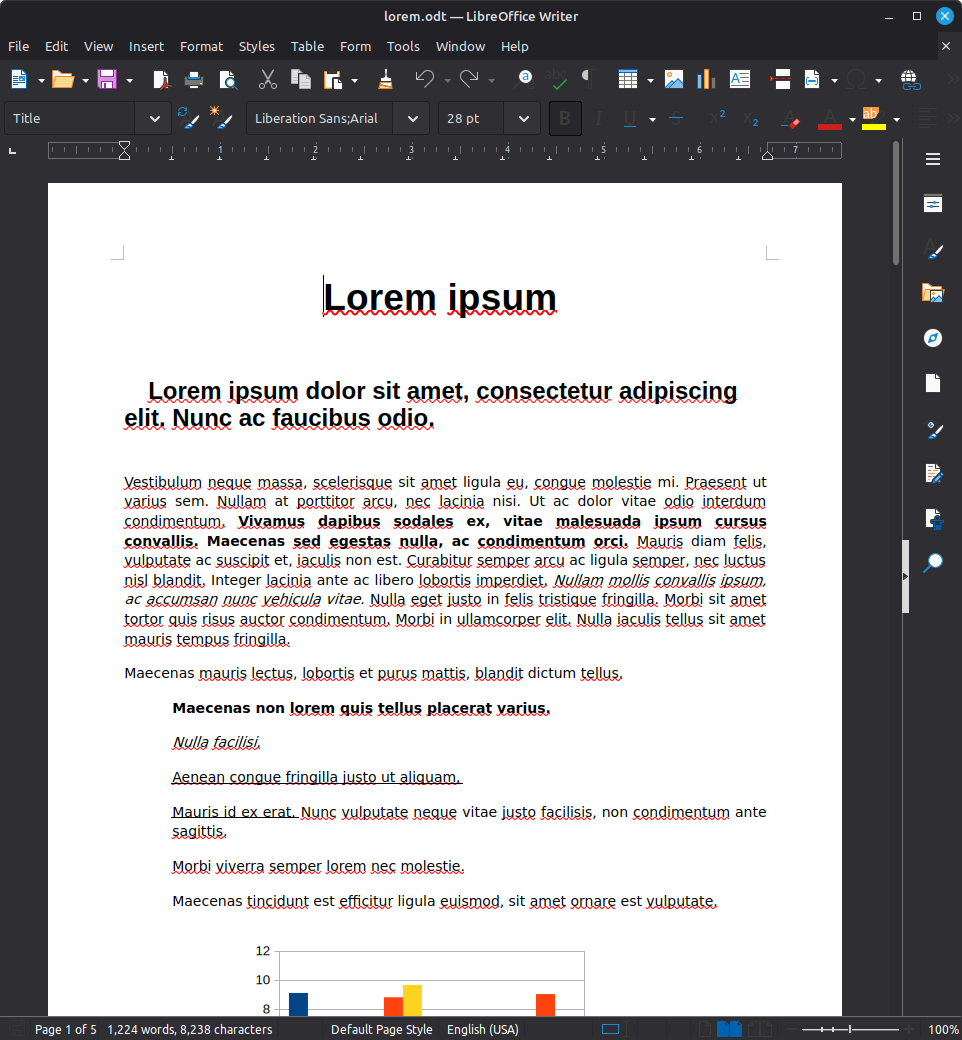
\includegraphics[width=0.95\linewidth]{assets/writer_screen.png}
    \end{column}
    \begin{column}{0.5\linewidth}
        \raggedleft
        \textbf{WYSIWYM}\par
        \vspace{0.3cm}
        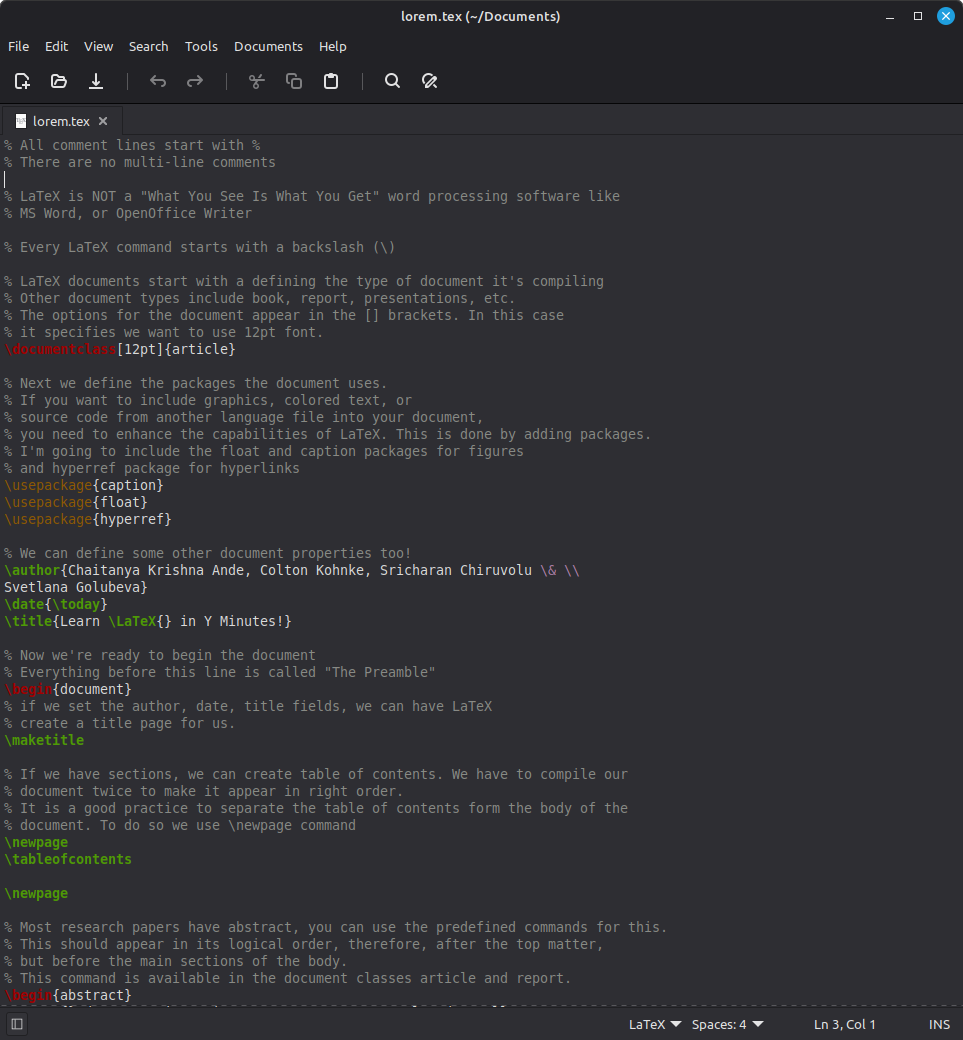
\includegraphics[width=0.95\linewidth]{assets/xed_screen.png}
    \end{column}
\end{columns}
\end{frame}


\begin{frame}
\begin{columns}
    \begin{column}{0.5\textwidth}
        \begingroup
        \centering \textbf{WYSIWYG}\\
        \textit{(What You See Is What You Get)}\\
        MS Word, Google Docs.\\
        \endgroup
        \vspace{0.3em}
        \begin{itemize}
            \item Formato visual inmediato.
            \item El autor se distrae con el diseño.
            \item Inestabilidad en documentos grandes.
        \end{itemize}
    \end{column}

    \begin{column}{0.5\textwidth}
        \centering \textbf{WYSIWYM}\\
        \textit{(What You See Is What You Mean)}\\
        {\lmr\LaTeX}, Markdown.\\
        \vspace{0.3em}
        \begin{itemize}
            \item El autor define la \textbf{estructura}.
            \item El sistema decide la \textbf{estética}.
            \item Formato ligero.
        \end{itemize}
    \end{column}
\end{columns}
\end{frame}



\begin{frame}[fragile]
\frametitle{Del Código al Papel}
\begin{columns}
    \begin{column}{0.45\textwidth}
        \begin{block}{Entrada (.tex)}
\begin{minted}{latex}
\section{Física Moderna}
La energía en reposo es:
\begin{equation}
  E = mc^2 \label{eq:eins}
\end{equation}
Como vemos en (\ref{eq:eins})
\end{minted}
        \end{block}
    \end{column}

    \begin{column}{0.1\textwidth}
        \centering $\rightarrow$
    \end{column}

    \begin{column}{0.45\textwidth}
        \begin{exampleblock}{Salida (.pdf)}
            \lmr
            \textbf{\Large 1. Física Moderna}\\
            \vspace{0.2cm}
            La energía en reposo es:
            \begin{equation*}
                E = mc^2 \quad (1)
            \end{equation*}
            Como vemos en (1)
        \end{exampleblock}
    \end{column}
\end{columns}
\end{frame}



\section{Pros y Contras}

\begin{frame}
\frametitle{¿Por qué sufrir con código?}
\begin{columns}
    \column{0.5\textwidth}
    \textbf{Ventajas:}
    \begin{itemize}
        \item Tipografía profesional (Kerning, ligaduras).
        \item Matemáticas perfectas.
        \item Gestión de bibliografía masiva.
        \item Automatización total de índices.
    \end{itemize}

    \column{0.5\textwidth}
    \textbf{Desafíos:}
    \begin{itemize}
        \item Curva de aprendizaje inicial.
        \item El diseño de plantillas es complejo.
        \item No hay revisión visual instantánea.
    \end{itemize}
\end{columns}
\end{frame}



\section{Anatomía de un Archivo \texttt{.tex}}
\begin{frame}[fragile]
\frametitle{La estructura mínima}
\begin{minted}{latex}
\documentclass[12pt]{article}

\title{Mi Primer Documento}
\author{PillFall}
\date{}

\begin{document}
\maketitle
¡Hola, Mundo {\LaTeX}!
\end{document}
\end{minted}
\end{frame}


\section{Motores y Distribuciones}
\begin{frame}
\frametitle{Motores y Distribuciones}
\begin{itemize}
    \item \textbf{Distribuciones:} TeX Live, MiKTeX, MacTeX (Mac).
    \item \textbf{Compiladores o Motores:}
    \begin{itemize}
        \item \texttt{pdflatex}: El estándar clásico. (Deprecado).
        \item \texttt{xelatex} / \texttt{lualatex}: Para usar cualquier fuente de tu PC.
    \end{itemize}

    \vspace{1em}
\end{itemize}
\end{frame}



\begin{frame}
\centering
{\Huge ¿Dudas?}
\vspace{1cm}
\begin{block}{Ejercicio}
    Descargar una distribución de {\lmr\LaTeX} y compilar nuestro primer documento.
\end{block}
\end{frame}

\begin{frame}[allowframebreaks]
\frametitle{Referencias}
\nocite{*}
\printbibliography
\end{frame}
\end{document}
